% questions.tex —— 2006 年·普通高等学校招生考试·福建卷文科 · 题目内容片段（无答案）
% 由 tools/generate_projects.py 依来源总账自 2006/2006_数学真题_福建文_试题.md 生成，勿手改（改源 MD 后重跑）


\begin{gktip}
\textbf{来源边界}：题签据固定 PDF 首页照录。题面按固定 PDF 第1—2页转录，印刷页码为290—291。该固定副本的发布者、出版者、版次、来源链及官方身份均未核实；来源清单中的 \texttt{ready} 仅代表固定候选文件通过格式检查，不是来源认证。固定 PDF 未见答案、解析或评分标准。
\textbf{转录说明}：题面按原页保留，未依题意修正或补全文字。Q10“对于平面 $\alpha$ 和共面的直线 $m\text{、}n$”的修饰范围不明确，按字面照录；Q19、Q20 示意图已按固定题面矢量重绘。
\end{gktip}

\gkpart{一、选择题}

\begin{question}
\gkti{1}已知两条直线 $y=ax-2$ 和 $y=(a+2)x+1$ 互相垂直，则 $a$ 等于\mbox{（　　）}

（A）$2$　　（B）$1$　　（C）$0$　　（D）$-1$

\end{question}
\begin{question}
\gkti{2}在等差数列 $\{a_n\}$ 中，已知 $a_1=2$，$a_2+a_3=13$，则 $a_4+a_5+a_6$ 等于\mbox{（　　）}

（A）$40$　　（B）$42$　　（C）$43$　　（D）$45$

\end{question}
\begin{question}
\gkti{3}“$\tan\alpha=1$”是“$\alpha=\dfrac{\pi}{4}$”的\mbox{（　　）}

（A）充分而不必要条件　　（B）必要而不充分条件

（C）充要条件　　（D）既不充分也不必要条件

\end{question}
\begin{question}
\gkti{4}已知 $\alpha\in\left(\dfrac{\pi}{2},\pi\right)$，$\sin\alpha=\dfrac35$，则 $\tan\left(\alpha+\dfrac{\pi}{4}\right)$ 等于\mbox{（　　）}

（A）$\dfrac17$　　（B）$7$　　（C）$-\dfrac17$　　（D）$-7$

\end{question}
\begin{question}
\gkti{5}已知全集 $U=\mathbb R$，且 $A=\{x\mid |x-1|>2\}$，$B=\{x\mid x^2-6x+8<0\}$，则 $(C_U A)\cap B$ 等于\mbox{（　　）}

（A）$[-1,4)$　　（B）$(2,3)$　　（C）$(2,3]$　　（D）$(-1,4)$

\end{question}
\begin{question}
\gkti{6}函数 $y=\dfrac{x}{x+1}\ (x\ne-1)$ 的反函数是\mbox{（　　）}

（A）$y=\dfrac{x}{1-x}\ (x\ne1)$　　（B）$y=\dfrac{x}{x-1}\ (x\ne1)$

（C）$y=\dfrac{x-1}{x}\ (x\ne0)$　　（D）$y=\dfrac{1-x}{x}\ (x\ne0)$

\end{question}
\begin{question}
\gkti{7}已知正方体外接球的体积是 $\dfrac{32}{3}\pi$，那么正方体的棱长等于\mbox{（　　）}

（A）$2\sqrt2$　　（B）$\dfrac{2\sqrt3}{3}$　　（C）$\dfrac{4\sqrt2}{3}$　　（D）$\dfrac{4\sqrt3}{3}$

\end{question}
\begin{question}
\gkti{8}从 $4$ 名男生和 $3$ 名女生中选出 $3$ 人，分别从事三项不同的工作，若这 $3$ 人中至少有 $1$ 名女生，则选派方案共有\mbox{（　　）}

（A）$108$ 种　　（B）$186$ 种　　（C）$216$ 种　　（D）$270$ 种

\end{question}
\begin{question}
\gkti{9}已知向量 $\vec a$ 与 $\vec b$ 的夹角为 $120^\circ$，$|\vec a|=3$，$|\vec a+\vec b|=\sqrt{13}$，则 $|\vec b|$ 等于\mbox{（　　）}

（A）$5$　　（B）$4$　　（C）$3$　　（D）$1$

\end{question}
\begin{question}
\gkti{10}对于平面 $\alpha$ 和共面的直线 $m$、$n$，下列命题中真命题是\mbox{（　　）}

（A）若 $m\perp\alpha$，$m\perp n$，则 $n\parallel\alpha$

（B）若 $m\parallel\alpha$，$n\parallel\alpha$，则 $m\parallel n$

（C）若 $m\subset\alpha$，$n\parallel\alpha$，则 $m\parallel n$

（D）若 $m$、$n$ 与 $\alpha$ 所成的角相等，则 $m\parallel n$

\end{question}
\begin{question}
\gkti{11}已知双曲线 $\dfrac{x^2}{a^2}-\dfrac{y^2}{b^2}=1\ (a>0, b>0)$ 的右焦点为 $F$，若过点 $F$ 且倾斜角为 $60^\circ$ 的直线与双曲线的右支有且只有一个交点，则此双曲线离心率的取值范围是\mbox{（　　）}

（A）$(1,2]$　　（B）$(1,2)$　　（C）$[2,+\infty)$　　（D）$(2,+\infty)$

\end{question}
\begin{question}
\gkti{12}已知 $f(x)$ 是周期为 $2$ 的奇函数，当 $0<x<1$ 时，$f(x)=\lg x$。设 $a=f\left(\dfrac65\right)$，$b=f\left(\dfrac32\right)$，$c=f\left(\dfrac52\right)$，则\mbox{（　　）}

（A）$a<b<c$　　（B）$b<a<c$　　（C）$c<b<a$　　（D）$c<a<b$

\end{question}
\gkpart{二、填空题}

\begin{question}
\gkti{13}$\left(x^2-\dfrac1x\right)^5$ 展开式中 $x^4$ 的系数是\gkblank{}。（用数字作答）

\end{question}
\begin{question}
\gkti{14}已知直线 $x-y-1=0$ 与抛物线 $y=ax^2$ 相切，则 $a=$\gkblank{}。

\end{question}
\begin{question}
\gkti{15}已知实数 $x\text{、}y$ 满足
\nopagebreak[4]
\[
\begin{cases}
y\le 1,\\
y\ge |x-1|,
\end{cases}
\]
则 $x+2y$ 的最大值是\gkblank{}。

\end{question}
\begin{question}
\gkti{16}已知函数 $f(x)=2\sin\omega x\ (\omega>0)$ 在区间 $\left[-\dfrac\pi3,\dfrac\pi4\right]$ 上的最小值是 $-2$，则 $\omega$ 的最小值等于\gkblank{}。

\end{question}
\gkpart{三、解答题}

\begin{question}
\gkti{17}已知函数
\nopagebreak[4]
\[
f(x)=\sin^2 x+\sqrt{3}\sin x\cos x+2\cos^2 x,\quad x\in\mathbb{R}.
\]

（1） 求函数 $f(x)$ 的最小正周期和单调增区间；

（2） 函数 $f(x)$ 的图象可以由函数 $y=\sin 2x\ (x\in\mathbb{R})$ 的图象经过怎样的变换得到？

\end{question}
\begin{question}
\gkti{18}每次抛掷一枚骰子（六个面上分别标以数 1，2，3，4，5，6）。

（1） 连续抛掷 2 次，求向上的数不同的概率；

（2） 连续抛掷 2 次，求向上的数之和为 6 的概率；

（3） 连续抛掷 5 次，求向上的数为奇数恰好出现 3 次的概率。

\Needspace{0.4\textheight}
\end{question}
\begin{question}
\gkti{19}如图，四面体 $ABCD$ 中，$O$、$E$ 分别是 $BD$、$BC$ 的中点，$CA=CB=CD=BD=2$，$AB=AD=\sqrt{2}$。

（1） 求证：$AO\perp$ 平面 $BCD$；

（2） 求异面直线 $AB$ 与 $CD$ 所成角的大小；

（3） 求点 $E$ 到平面 $ACD$ 的距离。
\nopagebreak[4]
\begin{center}% Schematic reconstruction of the visible Q19 diagram (2006 Fujian arts paper).
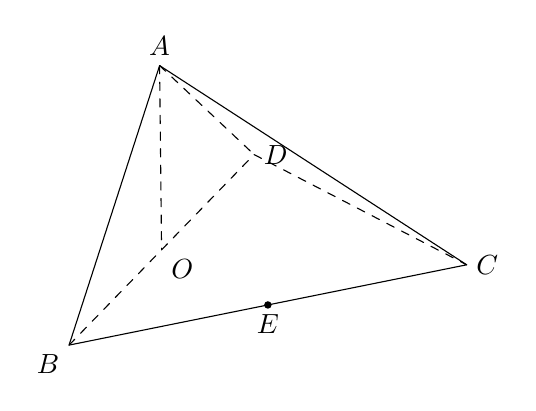
\begin{tikzpicture}[line cap=round,line join=round]
  % Schematic positions only; no lengths or angles are encoded.
  \coordinate (A) at (1.15,3.55);
  \coordinate (B) at (0,0);
  \coordinate (C) at (5.05,1.02);
  \coordinate (D) at (2.35,2.42);
  \coordinate (O) at (1.175,1.21);
  \coordinate (E) at (2.525,0.51);

  % Visible edges
  \draw (A) -- (B) -- (C) -- cycle;

  % Hidden edges and the indicated segment AO
  \draw[dashed] (A) -- (D);
  \draw[dashed] (B) -- (D);
  \draw[dashed] (D) -- (C);
  \draw[dashed] (A) -- (O);

  \fill (E) circle (1.35pt);
  \node[above]       at (A) {$A$};
  \node[below left]  at (B) {$B$};
  \node[right]       at (C) {$C$};
  \node[right]       at (D) {$D$};
  \node[below right] at (O) {$O$};
  \node[below]       at (E) {$E$};
\end{tikzpicture}
\end{center}
\nopagebreak[4]
\Needspace{0.4\textheight}
\end{question}
\begin{question}
\gkti{20}已知椭圆
\nopagebreak[4]
\[
\frac{x^2}{2}+y^2=1
\]
的左焦点为 $F$，$O$ 为坐标原点。

（1） 求过点 $O$、$F$，并且与椭圆的左准线 $l$ 相切的圆的方程；

（2） 设过点 $F$ 且不与坐标轴垂直的直线交椭圆于 $A$、$B$ 两点，并且线段 $AB$ 的中点在直线 $x+y=0$ 上，求直线 $AB$ 的方程。
\nopagebreak[4]
\begin{center}% Source schematic: 2006 Fujian arts paper, Q20, source PDF page 2.
% Include inside a document that loads TikZ.
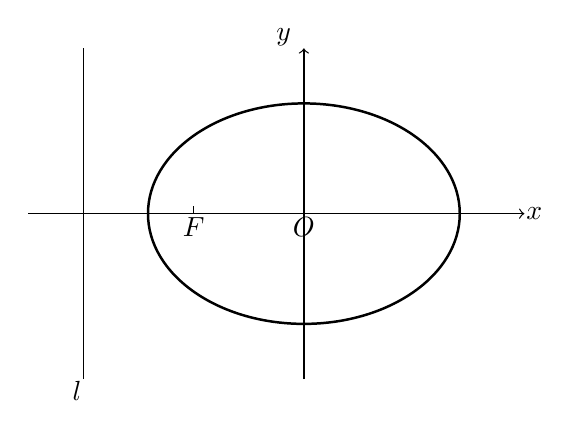
\begin{tikzpicture}[x=1.4cm,y=1.4cm,line cap=butt,line join=round]
  % Coordinate axes: arrows point in the positive directions only.
  \draw[->,line width=0.45pt] (-2.5,0) -- (2,0);
  \draw[->,line width=0.45pt] (0,-1.5) -- (0,1.5);

  % Left directrix, shown as a plain solid vertical line.
  \draw[line width=0.45pt] (-2,-1.5) -- (-2,1.5);

  % Ellipse x^2/2 + y^2 = 1, with the left focus tick on the x-axis.
  \draw[line width=0.9pt] (0,0) ellipse [x radius=1.4142,y radius=1];
  \draw[line width=0.45pt] (-1,0) -- (-1,0.07);

  % Labels copied from the schematic.
  \node[above left,inner sep=0.5pt] at (-0.1,1.5) {$y$};
  \node[right,inner sep=0.5pt] at (2,0) {$x$};
  \node[below,inner sep=0.5pt] at (-1,-0.02) {$F$};
  \node[below,inner sep=0.5pt] at (0,-0.02) {$O$};
  \node[below left,inner sep=0.5pt] at (-2,-1.5) {$l$};
\end{tikzpicture}
\end{center}
\nopagebreak[4]
\end{question}
\begin{question}
\gkti{21}已知 $f(x)$ 是二次函数，不等式 $f(x)<0$ 的解集是 $(0,5)$，且 $f(x)$ 在区间 $[-1,4]$ 上的最大值是 12。

（1） 求 $f(x)$ 的解析式；

\Needspace{5\baselineskip}
（2） 是否存在自然数 $m$，使得方程
\nopagebreak[4]
\[
f(x)+\frac{37}{x}=0
\]
在区间 $(m,m+1)$ 内有且只有两个不等的实数根？若存在，求出所有 $m$ 的值；若不存在，说明理由。

\end{question}
\begin{question}
\gkti{22}已知数列 $\{a_n\}$ 满足 $a_1=1$，$a_2=3$，$a_{n+2}=3a_{n+1}-2a_n\ (n\in\mathbb{N}^*)$。

（1） 证明：数列 $\{a_{n+1}-a_n\}$ 是等比数列；

（2） 求数列 $\{a_n\}$ 的通项公式；

\Needspace{5\baselineskip}
（3） 若数列 $\{b_n\}$ 满足
\nopagebreak[4]
\[
4^{b_1-1}4^{b_2-1}\cdots 4^{b_n-1}=(a_n+1)^{b_n}\quad(n\in\mathbb{N}^*),
\]
证明：$\{b_n\}$ 是等差数列。

\end{question}